\documentclass[11pts]{article}
\usepackage{geometry}
\usepackage[comma,sort&compress,numbers,sectionbib]{natbib}
\usepackage{url}
%\usepackage[scaled=1.0]{uarial}
\usepackage{graphicx}
\usepackage{wrapfig}
\usepackage[labelfont=bf]{caption}
\usepackage{bibentry}

\immediate\write18{bibtex \jobname}

% See the ``Article customise'' template for come common customisations
\begin{document}
\vspace{100 mm}
\title{Correlations between hypoxia and circulating cancer cells}
\author{Ching Kai Douglas Wu}
\date{Feburary 18, 2015 } % delete this line to display the current date
\maketitle
\bigskip


\section{Abstract} 
\noindent In pancreatic cancer, cells in solid tumors are supplied with different levels of oxygen depending on their distance from blood vessels. A fraction of tumor cells experience hypoxia. These cells adapt to a hypoxic environment by regulating hypoxia inducible factors (HIFs). Interestingly, recent work suggests hypoxia influences cancer cell dedifferentiation toward a stem-cell-like phenotype and promotes extracellular matrix (ECM) remodeling in cells, both of which are hallmarks for metastatic cells. During tumor metastasis, a number of tumor cells, circulating tumor cells (CTCs), are detectable in blood. However, the driving force of CTC formation is largely unknown. A recent study of single cell RNA-seq study of mouse CTC showed an increase in expression of hypoxia-induced factor (HIF-1$\alpha$) compared to primary tumor cells. This suggests that hypoxia may contribute to generation of CTCs in pancreatic cancer. In this work, I will test the hypothesis that tumor hypoxia promotes transformation of primary tumor cells to CTCs. I will investigate the up-regulation of hypoxia signaling and ECM remodeling proteins in circulating tumor cells. I will also study the relationship between hypoxia and CTC, by depleting HIF-1$\alpha$ locally at the tumor site. Furthermore, I will also study the effect of hypoxia on cell invasiveness. In summary, this work will provide insights into the effect of hypoxia on tumor progression, circulating tumor cell formation and understanding the driving force of metastasis. 
\newpage

\section{Specific Aims}
\noindent{\bf Aim 1. }Investigate up-regulation of molecules in the hypoxia signaling pathway.
\newline
\noindent{\bf Challenge} To test the hypothesis of hypoxia signaling up-regulation in circulating tumor cells compared to primary tumor cells.
\newline
\noindent{\bf Approach} I will use an established pancreatic tumor-bearing (KDC) mice as a tumor model. CTCs will be captured with CTC-iChip and differential expression will be assessed for HIF1 and hypoxia-related genes between CTCs and primary tumor cells by qRT-PCR and western blotting. 
\newline
\noindent{\bf Impact} As HIFs are regulated at the protein level, this experiment will further confirm the hypothesis that the hypoxia signaling pathway is activated in circulating tumor cells.
 \newline

\noindent{\bf Aim 2. }Identify the effects of hypoxia on CTC biogenesis and modifications of their ECM. 
\newline
\noindent{\bf Challenge} To test the hypothesis of hypoxia-induced-ECM gene regulation in pancreatic tumor cells. 
\newline
\noindent{\bf Approach} I will locally deplete HIF1 in pancreatic tumor cells by siHIF-1$\alpha$ LODER. Concentration of CTC will be monitored and single cell RNA-seq will be performed in order to track the ECM genes changes before and after treatment. 
\newline
\noindent{\bf Impact} This set of experiments will directly provide evidence on the role of HIF-1 in CTC generation in pancreatic tumor and will provide research direction to metastasis control in pancreatic tumor. 
\newline

\noindent{\bf Aim 3. }Investigate hypoxia-mediated enhanced extravasation of circulating tumor cells.
\newline
\noindent{\bf Challenge} To test the hypothesis that hypoxia influences CTC invasiveness.
\newline
\noindent{\bf Approach} CTCs collected from HIF1a-siRNA-treated tumors and control CTCs will be transferred to immunodeficient mice.
\newline
\noindent{\bf Impact} This would prove that a hypoxic tumor microenvironment not only drives intravasation of tumor cells and CTC production, but also improves their ability to extravasate and produce the next generation CTCs.
\bigskip

\section{Background and Significance}
\noindent{\bf Pancreatic ductal adenocarcinoma and metastasis}
\newline
\noindent Among solid tumors, pancreatic ductal adenocarcinoma (PDAC) is one of the most lethal. It is estimated that there will be 48,960 new cases and 40,560 deaths in 2015 \cite{CAAC:CAAC21254}. Although the 5-year survival rate is improving, it is still as low as 7\% \cite{CAAC:CAAC21254}. PDAC high mortality rate is due to its rapid rate of metastasis \cite{Ting:zl,23718921}. As described in {\it Hallmarks of Cancer}, metastasis is a multistage process. It consists of local invasion, intravasation, extravasation and colonization \cite{Hanahan2011646}.
\newline

\noindent Local invasion of tumor cells is evidenced by alteration of cell-cell and cell-extracellular matrix adhesion. A signature of local invasion is down-regulation of E-cadherin, a cell-cell adhesion molecule \cite{Hanahan2011646}. Intravasation describes the process by which a subtype of cells moves to nearby blood vessels or induces local angiogenesis within tumors \cite{Reymond:2013rw}. After intravasation, cells spread to distinct organs via the circulatory system and extravasate to new sites. From there, colonization of cells starts a new tumor \cite{Nguyen:2009qq}. 
\newline

\noindent{\bf Circulating tumor cells and cancer stem cells}
\newline
\noindent In between intravasation and extravasation, tumor cells travel within the circulatory system. These cells are extremely tumorigenic and are named circulating tumor cells (CTC) \cite{Alix-Panabieres:2014la}. It is proposed that CTCs can be indicators reflecting the increased risk of metastasis and tumor reoccurrence \cite{Noman:2014qf}. In spite of the important roles of CTCs in metastasis, it remains largely unknown how these cells are generated or selected, survive in the bloodstream, and invade distant organs.
  \newline

\noindent The cancer stem cell (CSC) theory is becoming more popular in cancer research as an explanation for the existence of CTCs and tumor reoccurrence. The CSC theory emphasizes an intratumor heterogeneity model in tumors, where tumor colonies consist of different subtypes of cells, one being a cancer stem cell \cite{Hanahan2011646}. These CSCs express markers of normal stem cells, are resistant to drugs, and most fatally, are capable of generating a new heterogeneous colony of tumor cells \cite{Hanahan2011646}. Due to the highly tumorigenic properties of CSCs, it is believed that a large fraction of circulating tumor cells is composed of cancer stem cells \cite{Noman:2014qf}. The mechanism that underlies intravasation of these cancer stem cells in solid tumor, like pancreatic ductal adenocarcinoma, is thought to be epithelial\textendash mesenchymal transition (EMT) \cite{Karamitopoulou:2012zr}. 
 \newline

\noindent{\bf Hypoxia, metastasis and epithelial-to-mesenchymal transition}
\newline
\noindent EMT is a part of regular developmental program that allows transition from epithelial to mesenchymal phenotype such as neuronal crest formation \cite{Noman:2014qf,Singh:2010ys,Hanahan2011646}. A signature of EMT is the down-regulation of cell-cell interactions as these cells become more motile \cite{18566898}. In epithelial cancers like PDAC, it is known that circulating tumor cells exhibit mesenchymal phenotypes and stem cell-like properties \cite{Rhim:2012fk}. This implies that EMT plays an important role in metastasis. This is further supported by an {\it in vitro} study using a pancreatic cancer cell line, which showed that hypoxia-induced EMT drives the migratory potential and intravasation of cancer stem cells, suggesting these EMT-CSCs are ideal candidates for circulating tumor cells \cite{10.1371/journal.pone.0046391}. 
\newline

\noindent Interestingly, apart from EMT, hypoxia also plays a role in extracellular matrix (ECM) remodeling of tumor cells, a crucial element of intravasation \cite{Gilkes:2014qf}. A typical example of downstream effector of hypoxia is collagen I, which involves in a physical and biochemical role in the tumor microenvironment and promotes tumor progression \cite{Gilkes:2014qf}. For example, intratumor hypoxia induces degradation of extracellular proteins by up-regulation of matrix metalloproteinase and directly promotes tumor invasion \cite{Krishnamachary:2003vn,MC:MC20678}.
 \newline

\noindent{\bf Hypoxia-induced factors and hypoxia signaling}
\newline
\noindent Intratumoral hypoxia occurs in areas with low oxygenation (\textless10 mmHg) and in areas often distant from blood vessels and vascular networks \cite{Gilkes:2014qf}. Cells respond to hypoxia by the activity of hypoxia-inducible factors 1 (HIF-1) \cite{10.1172/JCI67230}. HIF-1 is a heterodimer of HIF-1$\alpha$ and HIF-1$\beta$. Between these two subunits, HIF-1$\alpha$ is constitutively expressed and is a nuclear translocator while HIF-1$\alpha$ is oxygen-regulated \cite{10.1172/JCI67230}. HIF-1$\alpha$ contains an oxygen-dependent degradation domain (ODD) that is regulated by HIF prolyl-4-hydroxylases, which are 2-oxoglutarate- and iron-dependent enzymes that hydrolyze two proline sites on the ODD \cite{Karuppagounder:2012sf}. Under normoxic conditions, hydroxylation of HIF-1$\alpha$ induces binding to the Von Hippel Lindau tumor suppressor protein and will be recognized by an E3 ubiquitin ligase complex. Hydroxylated HIF-1$\alpha$ is thus poly-ubiquitinated at the ODD domain and directed to the proteosome for degradation \cite{Karuppagounder:2012sf}.\newline

\noindent HIFs are master regulators for genes that involved in angiogenesis and tumor growth, including vascular endothelial growth factor (VEGF) and transforming growth factor-beta (TGF-$\beta$). Besides regulation of angiogenesis and metabolism, it is reported that the transcriptional activity of the HIF-1$\alpha$/HIF-1$\beta$ heterodimer also promotes a stem cell-like phenotype in cells \cite{Noman:2014qf,10.1172/JCI67230}. This raises the question on whether HIF1 and hypoxia contribute to circulating tumor cells generation. Additionally, hypoxia might also increase the invasiveness of these CTCs. 
\newline

\noindent{\bf Proposed Work}
\newline
\noindent In this proposed work, I will address the hypothesis that CTCs generation, intravasation and extravasation are promoted by hypoxia-induced adaptive changes in the tumor mass instead of being a spontaneous process. In my first aim, I will investigate hypoxia signaling levels in CTCs. I will capture CTCs in pancreatic-tumor-bearing mice and compare expression level of hypoxia signaling proteins and ECM proteins between CTCs and the primary tumor. A recent {\it in vivo} single cell RNA-seq study revealed increased expression of a stromal-derived ECM protein-coding gene in circulating tumor cells \cite{Ting:zl}. Using the data in this single cell RNA-seq study, up-regulation of HIF-1$\alpha$ in circulating tumor cells can be seen with a p-value \textless 0.05 (figure 1). However, as HIF-1 is highly regulated post-translationally, it would be necessary to measure the HIF-1$\alpha$ protein expression levels in CTCs \cite{Wenger:1997fk}.
 \newline

\noindent On the other hand, I also hypothesize blocking the hypoxia signaling pathway will delay metastasis in an {\it in vivo} mouse model of pancreatic cancer. Although heterogeneity of cells in CTC has been reported, I hypothesize hypoxia is the major driving force of intravasation of these cells regardless of phenotype. In order to test this hypothesis, I will suppress HIF-1 in primary tumors and capture any changes in CSC number and ECM gene expression levels compared to untreated mice. This experiment will further identify hypoxia as a regulator of cancer metastasis and support tumor drug development against HIF-1.
 \newline

\noindent Moreover, as {\it in vitro} experiments have shown that hypoxia increases the invasiveness of EMT pancreatic cells \cite{10.1371/journal.pone.0046391}, I will also capture CTCs {\it in vivo} from the pancreatic cancer model mice and investigate their ability to extravasate. I will compare CTCs in HIF-1 knock down mice to those from untreated mouse. This will identify the effect of hypoxia in {\it in vivo} pancreatic tumor cells. 
 \newline

\noindent{\bf Significance}
\newline
\noindent The proposed work will provide an extensive framework on the relationship between hypoxia and circulating tumor cells by directly investigating the role of hypoxia in pancreatic tumor progression. Similar models can be developed for other solid tumors and this research supports drug development against HIF-1$\alpha$ for treating metastatic tumors. This work will also potentially provide new insights into the different signaling pathways driving metastasis and EMT in solid tumors. 
\newline


%==============================aim 1=========================
\section{Approach}
\noindent {\bf Aim 1.  Investigate up-regulation of molecules in hypoxia signaling pathway. }
\newline
For this aim, I will use an established pancreatic tumor mouse model, LSL-Kras$^{G12D}$, Trp53$^{flox/flox}$, Pdx1-Cre (KPC) mouse, which is known to produce CTCs \cite{Bardeesy:2006xy,Rhim:2012fk,Ting:zl}. The same mouse line has been used for CTC single cell sequencing, and the data showed a higher RNA expression of hypoxia-induced factor 1 alpha subunit in circulating tumor cells than in primary tumor cells\cite{Ting:zl}. I will use a well-characterized micro-fluidic device, CTC-iChip, to isolate CTCs from collected whole blood cells \cite{Ting:zl}. 
\newline

\noindent In order to isolate nucleated cells from red blood cells as well as platelets and plasma, CTC-iChip utilizes size-based separation (figure 2). Moreover, as leukocytes will be labeled with anti-CD45-conjugated magnetic beads, CTCs can be enriched with magnetic cell sorting \cite{Ting:zl}. As previously suggested, I would expect to collect around 150 CTCs from 1-ml of blood by CTC-iChip \cite{Ting:zl}.
 \newline


\noindent After cells are sorted, I will lyse the cells and use monoclonal HIF-1$\alpha$ antibody for western blotting. I will compare the expression level of HIF-1$\alpha$ protein between circulating tumor cells and primary tumor cells from the same mouse using $\beta$-actin as control. As HIF-1$\alpha$ have a half-life of 5-min in cytoplasm under normoxic conditions and blood vessels are well-oxygenated, I will compare the expression level of HIF-1$\alpha$ in the nuclear extracts \cite{Karuppagounder:2012sf}. This is also reasonable since HIF-1$\alpha$ has a transcription factor activity in the nucleus. 
\newline

\noindent For this experiment, I anticipate to see bands at around 116 kDa with higher intensity for CTC samples. This will indicate a higher HIF-1$\alpha$ expression in circulating tumor cells than in primary tumor and implies hypoxia signaling is up-regulated in circulating tumor cells. It will also suggest hypoxia maybe the driving force of intravasation of tumor. 
\newline

\noindent In addition to HIF-1$\alpha$ protein, I will use RT-PCR to confirm the up-regulation of hypoxia signaling molecules in CTC samples by Hypoxia Signaling Pathway PCR Array. This will simultaneously test 96 hypoxia related genes including HIF-1 and co-transcription factors, other HIF-1 interactors and HIF-1 responsive genes. I predict that higher expression level of hypoxia responsive genes and stable expression of HIG-1 interactors and co-transcription factors, since HIF-1 is the only oxidation-responsive molecule in the pathway. Molecules that are differentially regulated will indicate that hypoxia in primary tumors can selectively activate certain pathways. 
\newline

\noindent There is a potential pitfall for detecting differential expression level of HIF-1 since HIF-1$\alpha$ is regulated post-translationally. The activity of HIF-1 may not be merely reflected by the abundance of HIF-1$\alpha$ and CTCs might express HIF-1$\alpha$ protein at the same level as primary tumors. 
\newline

\noindent An alternative approach is to establish tumor xenografts in nude mice with human pancreatic tumor cell line that stably expressing ODD-GFP (oxygen-dependent degradation domain fused with green fluorescent protein) and measure GFP signals in captured CTCs \cite{DAngelo:2003fj}. ODD-GFP reporter gene expresses GFP with a HIF-1$\alpha$ oxygen-dependent degradation domain. Under normoxia condition, HIF prolyl-4-hydroxylases induce degradation of the protein and GFP fluorescence is lost. This will enable the identification of CTCs with active HIF-1$\alpha$-active cells in CTCs. Moreover, I can also preform HIF-1$\alpha$ immunofluorescence staining in the collected cells. Combining with nuclear staining, this will further enable visualization of HIF-1$\alpha$ spacial distribution in CTCs and primary cancer cells. 
\newline

\noindent The results of this experiment will confirm the hypothesis that circulating tumor cells possess a hypoxic phenotype. This will show hypoxia signaling is up-regulated in circulating tumor cells and suggest hypoxia might be the driving force for intravasation of circulating tumor cells.
\newline

\noindent {\bf Aim 2. Identify the effect of hypoxia in CTC generations and ECM modifications in CTC}
\newline
\noindent For this aim, I will deplete HIF-1$\alpha$ in the KPC pancreatic tumor mouse model to evaluate the effect of hypoxia in circulating tumor cells generation and differential expression of ECM remodeling factors. I will use a local prolonged siRNA delivery system, Local Drug EluteR (LODER), to deliver 10-$\mu$g HIF-1$\alpha$ siRNA into pancreatic tumor site \cite{Zorde-Khvalevsky:2013fk}. LODER will be implanted in the pancreatic tumor directly using a 19-gauge endoscopic ultrasound needle to protect the siRNA from degradation. HIF-1$\alpha$ siRNA will be released in the local tumor microenvironment. This ensures that hypoxia signaling is only inhibited at the pancreatic tumor site.
 \newline

\noindent I will use two groups of KPC mice: one treated with siHIF-1$\alpha$ LODER while the other group is untreated.  I will collect 1-ml of blood weekly from each group starting at 5 weeks old and I extract CTCs from blood cells and other components in blood using CTC-iChip. The number of CTCs collected in a milliliter of blood will be recorded for each collection and time point to determine if depleting HIF-1$\alpha$ has a significant effect on reducing the number of circulating tumor cells. 
\newline

\noindent In addition to CTC counts, I will also repeat the single cell RNA-seq experiment on these cells \cite{Ting:zl}. I will sequence 150 cells per sample and profile the gene expression of these cells. I will perform gene ontology enrichment analysis (GO analysis) for differentially expressed genes and determine the pathways that have been knocked down. For any important findings such as differentially expressed master regulators, I will perform RT-PCR to confirm the result.  
\newline

\noindent As inhibiting hypoxia signaling will impair cells from adapting to hypoxia, I would expect a decrease in number of CTCs being captured in siHIF-1$\alpha$ LODER-treated mice. This is because HIF-1$\alpha$ regulates VEGF, causing an increase in angiogenesis, TGF-$\beta$ for proliferation and EMT regulators such as, Twist1, Snail and Slug. I would also predict to see differential expression of ECM genes as well as those related to angiogenesis and EMT \cite{Pugh:2003kx}. HIF-1$\alpha$ RNA will act as a control in this experiment because there should be little to no HIF-1$\alpha$ mRNA being captured in RNA-seq for CTCs from siHIF-1$\alpha$ LODER treated mice. 
\newline

\noindent From the RNA-seq data, I also expect to see CTC heterogeneity from both siRNA-treated and untreated samples. It would be interesting to determine if there are different CTC subtypes between samples. In addition, if any new subtypes of CTCs are observed compared to the published datasets \cite{Ting:zl}, it might suggest a different signaling pathway has replaced hypoxia in HIF-1$\alpha$ depleted tumors to regulate CTC generation. 
\newline

\noindent A potential failure of this set of experiments would be implantation error of LODER into the pancreatic tumor. Positive controls for correct implantation would include using siG12D LODER as described previously, which down-regulates Kras and leads to an easily-visualized larger necrotic area in the tumor after 1 week  \cite{Zorde-Khvalevsky:2013fk}.  I will also include a negative control experiment with empty LODER in order to ensure that LODER alone does not have any impact on the tumor. With these two controls, I will be able to assess the experimental setup and validate the finding from the experimental subjects. An alternative experiment can be carried out by collecting CTCs from tumor xenografts generated with HIF-1$\alpha$ knock-out pancreatic tumor cells in nude mice.   
\newline

\noindent The result from this aim will directly address the question of whether hypoxia is the driving force of circulating tumor cells generation and assess if hypoxia is necessary and sufficient to drive tumor metastasis. As all biological pathways are composed of gene networks, I would not expect the complete inhibition of CTC generation after depleting of HIF-1$\alpha$. 
\newline

\noindent The result here can also be used as a future reference. The single cell RNA-seq datasets from this aim can be mined to identify signaling pathways that have been altered. On the other hand, the datasets should also be useful for mining post-transcriptional modification changes in HIF-1$\alpha$-depleted CTCs. This may provide insights on CTC signaling pathways, induction mechanisms of EMT, as well as CTC biogenesis itself.
 \newline

\noindent {\bf Aim 3. Investigate hypoxia-mediated enhanced extravasation of hypoxia in circulating tumor cells. }
\newline
\noindent For this aim, I will use the same techniques as in Aim 2 to setup my control group and experimental group of cells. I will apply siHIF-1$\alpha$ LODER to mice and collect CTCs from blood using CTC-iChip. The cells will be injected into nude ((NOD)-SCID IL2r$\gamma^{-/-}$) and wild type mice (C57BL/6J) to test their ability to initiate new tumors. Nude mice are severe combined immunodeficiency mice, they can be models for extravasation of circulating tumor cells. I will use nude mice as the experimental subjects. 
\newline

\noindent To evaluate the ability of transplanted CTCs to generate new tumors, I will inject a dilution series of these cells into both groups of mice. As a method of comparison, I will monitor tumor growth by size daily, and measure their morphology and mass at one month. Additionally I will measure daily CTC counts. 
\newline

\noindent As HIF-1$\alpha$ induces ECM remodeling and it has been shown that hypoxic conditions select for aggressive phenotypes in tumors \cite{Ameri:2010qf}, I predict more CTCs from HIF-1$\alpha$ depleted mice are required to generate tumors in both SCID and wild-type recipients when compared to CTCs from untreated donor mice. Moreover, I anticipate observing larger tumor size and mass in recipient mice injected with CTCs from untreated donor mice. SCID and wild-type mice would also be predicted to have higher CTC counts themselves when injected with CTCs from untreated donor mice. \newline

\noindent I will include normal mice in the experiment to test the tumorigenicity of the isolated CTCs. Others have reported that in the case of some extremely tumorigenic cells, injection of as few as ten of such cells can lead to tumor formation in wild type mice \cite{Liu:2012ys}. I expect this unconventional experiment can differentiate the tumorigenicity of CTCs from siHIF-1$\alpha$ treated mice and untreated mice. Moreover, this experiment would also enable the understanding on the effect of hypoxia on immuno escape of circulating tumor cells. 
 \newline

\noindent Since the concentration of CTCs in blood is low, each mouse might not have sufficient CTCs for injection. To overcome this limitation, I will combine CTCs from the same test group. As mice from the same group are treated in the same way, there should not be any bias regarding tumor initiation in immunodeficient mice. \newline

\noindent An alternative approach involves seeding captured CTCs in cell culture wells and monitoring their ability to initiate cell mass in 3D matrigels. This method would also enable the comparisons of tumorigenicity between HIF-1$\alpha$-depleted and normal CTCs. 
\newline

\noindent If the expected results are observed, this would support my hypothesis that a hypoxic tumor microenvironment not only drives intravasation of tumor cells and CTC production, but also improves the ability of CTCs to extravasate and produce next generation CTCs. 
\newline

\noindent As an additional experiment, I can also culture the isolated CTCs from wild-type and SCID mice in hypoxia environment and inject into mice. It was shown in breast cancer cell line that CTCs exposed to hypoxia again are more aggressive than tumor that is exposed to hypoxia once \cite{Ameri:2010qf}. It will be interesting to use this experiment to observe the hypoxia response of temporary-HIF-1$\alpha$ knocked-down CTCs. This will potentially help understand and predict secondary tumor metastasis from CTC phenotypes and improve metastatic predictions in solid tumors. 
 \newline



\section{Reference}
%\begingroup
\renewcommand{\section}[2]{}
{%\footnotesize
\bibliographystyle{myNatBibStyle}
\setlength{\bibsep}{2.0pt}
\bibliography{wu_C_hypoxia}}
%\endgroup
\newpage


\begin{wrapfigure}{R}{1\textwidth}
\centering	
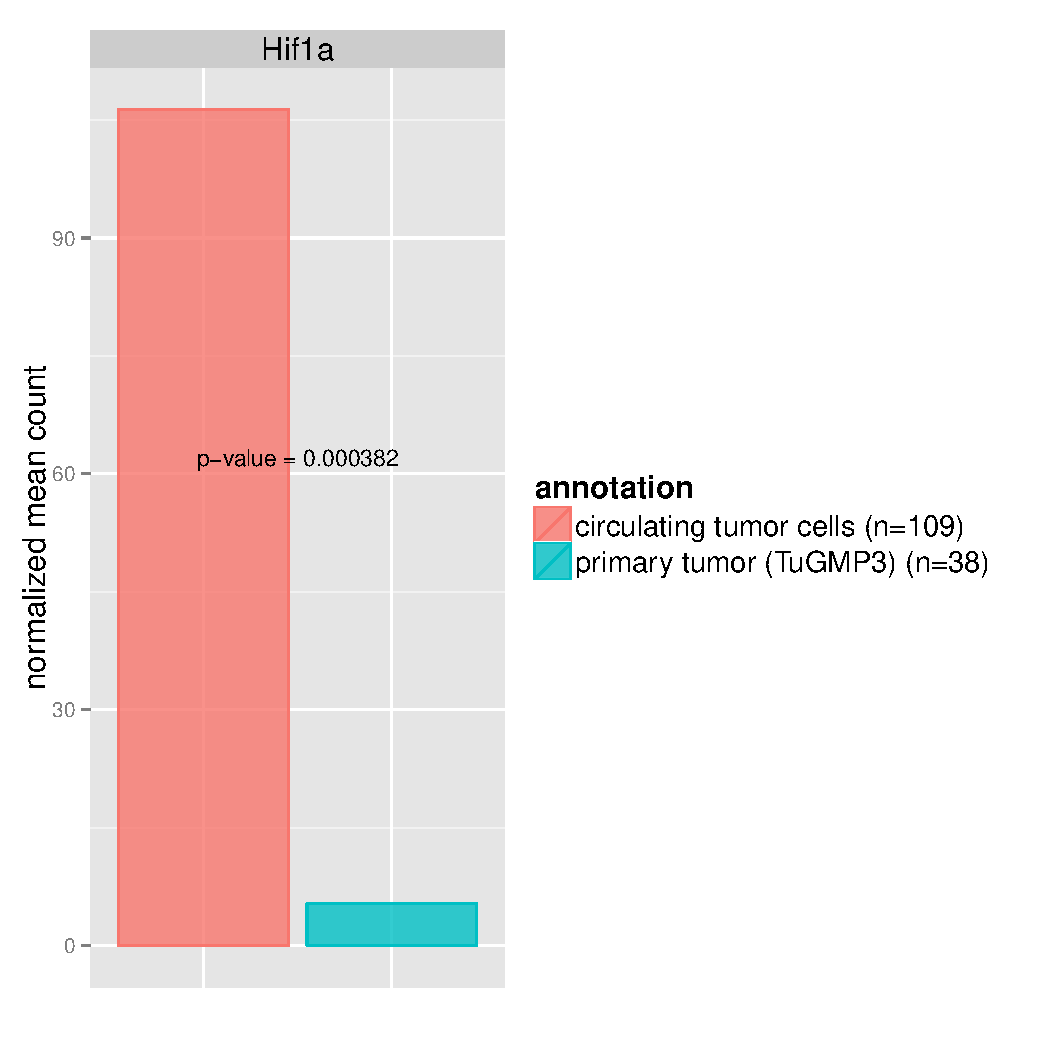
\includegraphics[width=1\textwidth]{qualexam_HIF.pdf}
\caption{\small {\bf Expression level of HIF-1$\alpha$ and HIF-1$\alpha$ inhibitor in circulating tumor cells versus primary tumor cells. } RNA expression level of HIF-1$\alpha$ and HIF-1$\alpha$ inhibitor from mouse CTC and primary tumor cells single cell RNA-seq data is compared in the bar graph  [2]. The expression level of HIF-1$\alpha$ is significantly higher in CTCs than that of primary tumor cells while inhibitor of HIF-1$\alpha$ is not differentially expressed significantly. It implies hypoxia signaling might have been activated and up-regulated in circulating tumor cells both transcriptionally and translationally.   } 

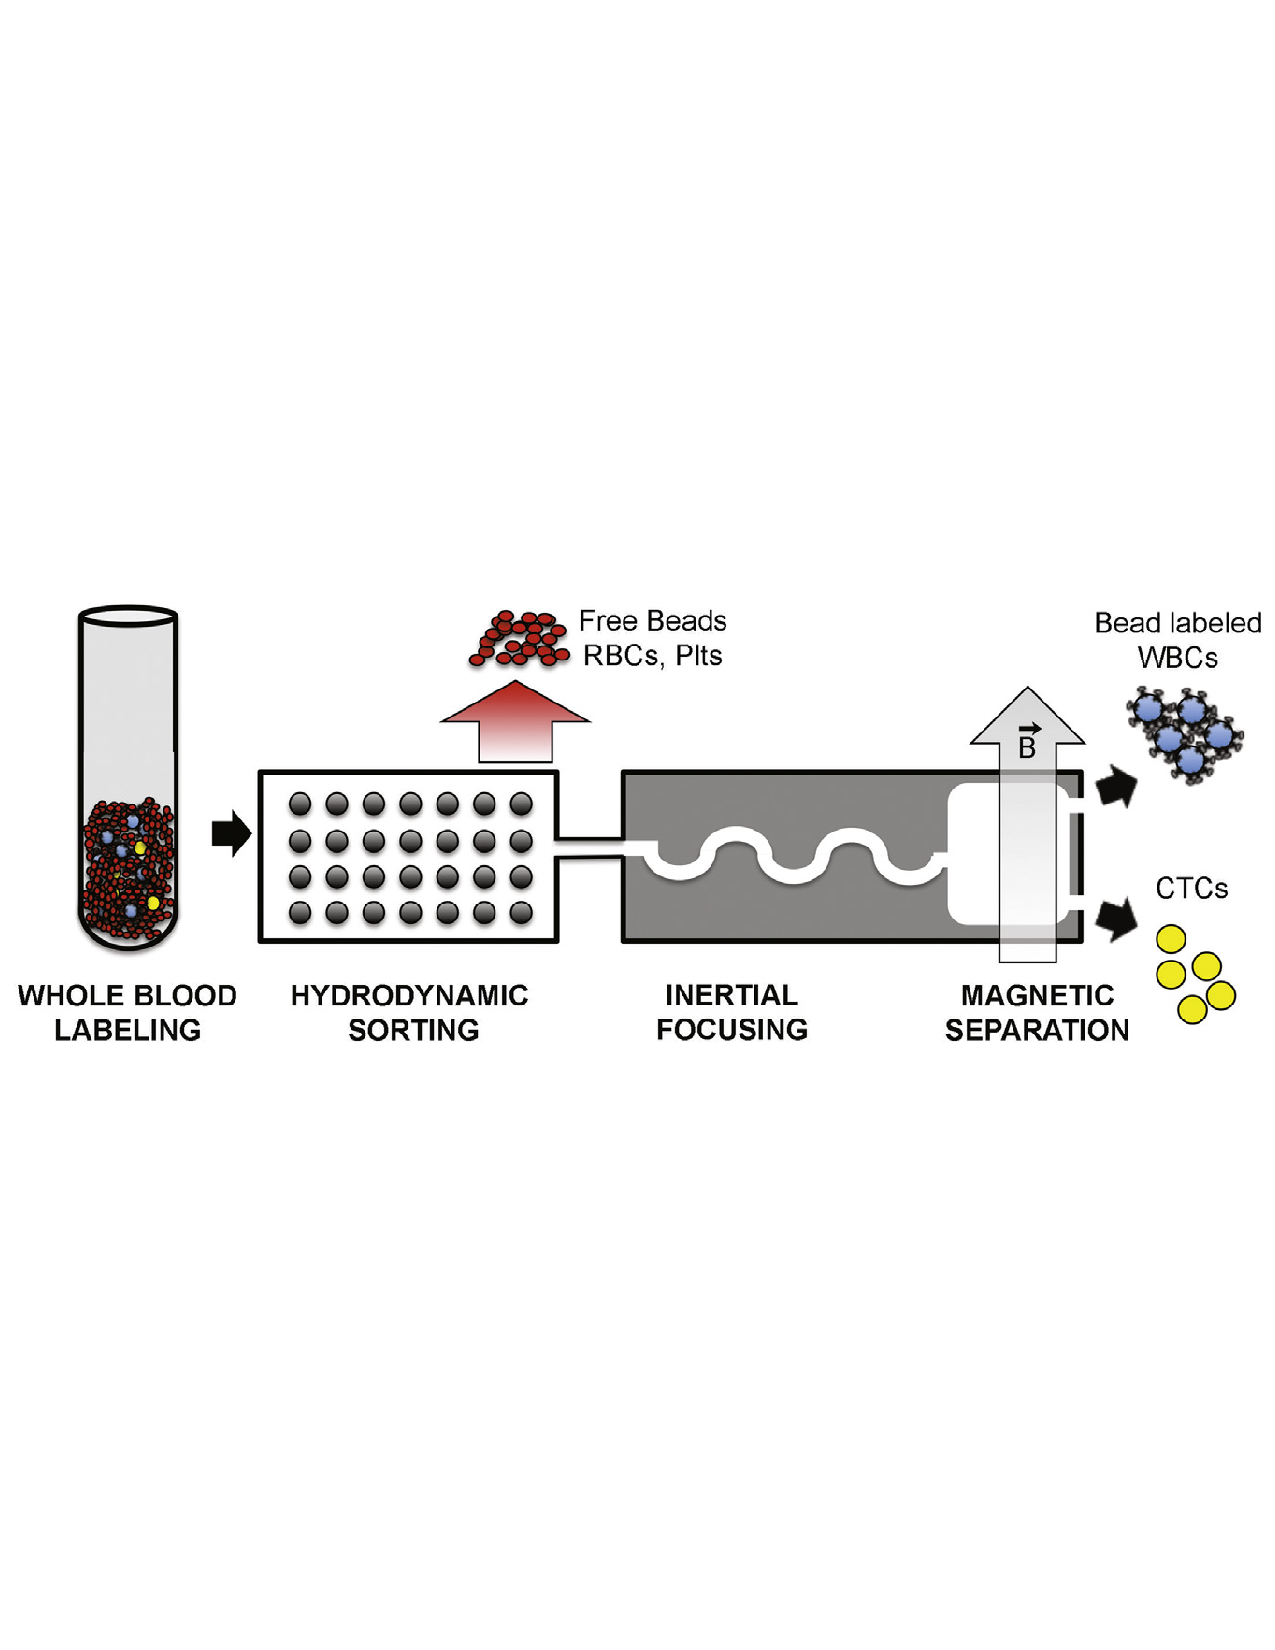
\includegraphics[width=1\textwidth]{ichip.pdf}
\caption{\small {\bf Schematic of CTC selection from blood using CTC-iChip. } This figure described the strategy of CTC selection device implied in this proposed study. Magnetic beads, conjugated with CD45 and CD66b antibody, are mixed with cells and labeled leukocytes and granulocytes. All cells are then separated by size using nano-poles to filter out molecules that have diameter \textless 4$\mu m$ (red blood cells, blood platelets, free antibodies and magnetic beads). After that, the remaining cells are separated by magnetic field in order to enrich CTCs. Figure adapted from Ting, {\it et al.} [2]. } 
\end{wrapfigure} 


\end{document}
